\documentclass[11pt,final] {article}
\usepackage[margin=1in]{geometry}
\usepackage{tikz}
\usepackage{amsmath}
\usepackage{float}
\usepackage{fancyvrb}
\usepackage[margin=1in]{geometry}
\usepackage{fancyhdr}
\usepackage{graphicx}
\usepackage{makeidx}
\usepackage{color}
\definecolor{darkblue}{rgb}{0,0,0.5}
\usepackage{hyperref}
\hypersetup{colorlinks,
	linkcolor=darkblue,
	filecolor=darkblue,
	citecolor=darkblue,
	urlcolor=blue}

%%%%%%%%%%%%%%%%%%%
% Other opts and styling
%%%%%%%%%%%%%%%%%%%

\graphicspath{{./assets/}}

\pagestyle{fancy}
\renewcommand{\headrulewidth}{0pt}
\fancyhead{}
\fancyfoot{}
\rhead{\thepage}

%%%%%%%%%%%%%%%%%%%
% Start content
%%%%%%%%%%%%%%%%%%%
\begin{document}

\section{Standard Deviation}
\textbf{Standard deviation} \index{Standard deviation} (represented as $s$ or $\sigma$) is a measure of dispersion: that is, it tells us how far from or close to the mean our data tend to be. A dataset with a small standard deviation, for instance, tells us that most of our data points are fairly close together and are all near the mean. Alternately, a large standard deviation means that our data points are much more spread out. We can visualize this using three data sets, all with mean $\mu=0$ but with different standard deviations, as in Figure \ref{fig:uncertainty03}.

\begin{figure}[htp]
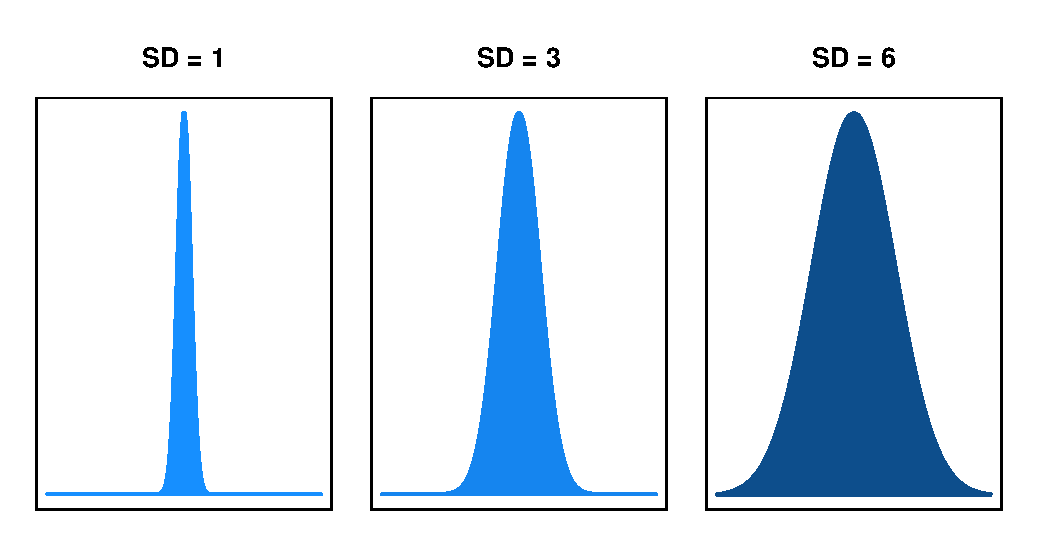
\includegraphics[width=35pc]{uncertainty03}
\caption{Three samples of data with mean \(\mu=0\) and standard deviations of 1, 3, and 6, respectively.}
\label{fig:uncertainty03}
\end{figure}

Even though each of these three sets of data has the same mean (0), it's pretty clear that there are some big differences between each of them. This is why standard deviation is important to know and report: without it, you aren't going to be getting a complete picture of what your data look like. They could all be close to the mean, as in the graph on the far left, or they could be much more spread out, as in the graph on the right.

Now, before we can use standard deviations, we have to calculate them. The formula for standard deviation looks like:

\begin{equation}
\sigma = \sqrt{
	\frac{1}{n}\sum_{i=1}^n\left(x_i-\mu\right)^2
	} \text{, where }
	\mu=\frac{1}{n}\sum_{i=1}^n(x_i)
\end{equation}

Let's unpack that: it's saying that we start by finding the mean ($ \mu $) of the data. Next, we'll go ahead and take every data point and subtract the mean from it (the $ x_i-\mu $ part of the equation). So what we're doing is basically finding out how many units away from the mean each data point is. But there's a problem: some data points might give us a negative number, others a positive number. So we'll take that difference and raise it to the second power (remember, a negative number times a negative number is always equal to a positive number). Now we just repeat that for every other data point in our sample and add them all together.

So now we have summed up all of those squared differences, right? Next, we will divide by the number ($ n $) of observations (just like when we calculated the mean) to get the \textbf{average distance from the mean}. But there's one last step before we're done: since we raised everything to the second power a couple steps ago, we have to undo that operation. To do this, we'll take the square root of everything, leaving us at last with the standard deviation.

Now, it's also important to note the difference between a {\bfseries sample standard deviation} and the {\bfseries population standard deviation}. The former (represented $s$) is what we deal with when we run experiments. The population mean ($\mu$) exists, but it's really unlikely that we can ever know what it is. The idea is that if we take a measurement from every possible subject or cell culture, etc. (literally, an infinite number of them), there will be one final mean to rule them all. That's the population mean. That's hard to figure out.

Instead, we have sample means to rely on. The formula is pretty similar to the one above:

\begin{equation}
\sigma = \sqrt{
	\frac{1}{n}\sum_{i=1}^n\left(x_i-\bar{x}\right)^2
	} \text{, where }
	\bar{x}=\frac{1}{n}\sum_{i=1}^n(x_i)
\end{equation}

Here, we're taking a random sample of size $n$ from the population as a whole. This means that, although the mean and standard deviation will likely (as a result of our random selection) be close to those of the population, they {\bfseries will not be identical}. There's always going to be some little pesky amount of purely random variation thrown into the mix.

\section{Sampling Distributions}

\subsection{Central Limit Theorem and Sampling Distributions}
Does the central limit theorem ring any bells? Probably not. But it's still probably something that you've heard of before. Specifically, you may have heard of it in the context of \textbf{regression to the mean} \index{Regression to the mean}. This is the idea that (let's use height as an example) if you randomly choose one adult male in the U.S., his height could very easily be 7'3". That's obviously a lot taller than most people. But the next person you choose will probably have a height less than the first guy's. And if you keep choosing more and more people and measuring their heights, pretty soon, the average height of everyone you chose will be pretty darned close to the actual national average height for adult males. More generally, the idea is that every now and then there will always be extreme scores. But every time you get one of those strong outliers, the next observation is almost certainly going to be less extreme and it is going to pull things back down to the population average.

The \textbf{central limit theorem} \index{Central limit theorem} is sort of similar: it states that the distribution of an average tends to be normal, even if the population is not itself normal.

Make sense? Maybe not (that's okay!), so let's break it down a bit. Whenever we're talking about a distribution of averages, we call that a \textbf{sampling distribution} \index{Sampling distribution}. To continue with our height example from above, let's say that we randomly choose 25 guys and measure their heights. Then we choose another 25 guys and measure their heights. Then we choose another 25 guys and measure their heights. Assuming that the mean male adult height is 5'8" with a 4" standard deviation (we have to represent that with decimals in R, so it becomes a mean of 5.67 feet and a standard deviation of 0.33 feet), our three samples might look like Figure \ref{fig:uncertainty05}.

\begin{figure}[h!]
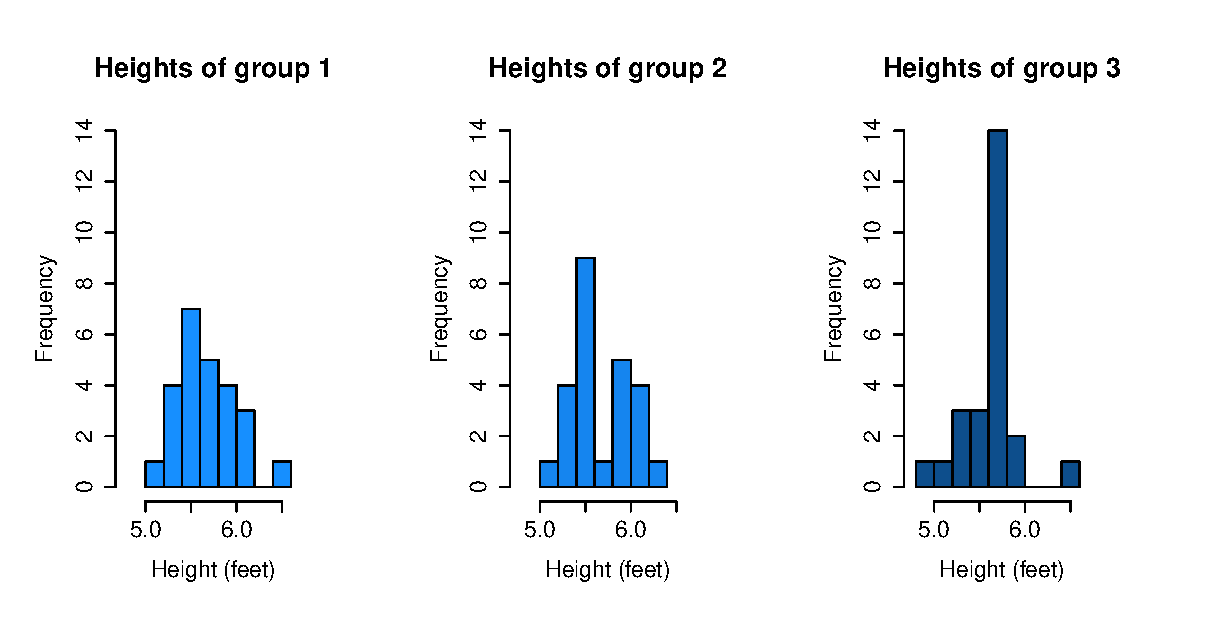
\includegraphics[width=35pc]{uncertainty05}
\caption{Heights of three randomly-selected groups of men}
\label{fig:uncertainty05}
\end{figure}

We can see that there's a lot of variation among our three groups, right? And groups 2 and 3 don't really look all that normal. But, let's say that we take the average male height of each of our three samples. Now, let's repeat that with another 497 batches of 25 men each. Now, for each of those 25-person samples, let's take their average. If we make a histogram of the average height from each of those 500 groups, it will look like Figure \ref{fig:uncertainty06}.

\begin{figure}[h!]
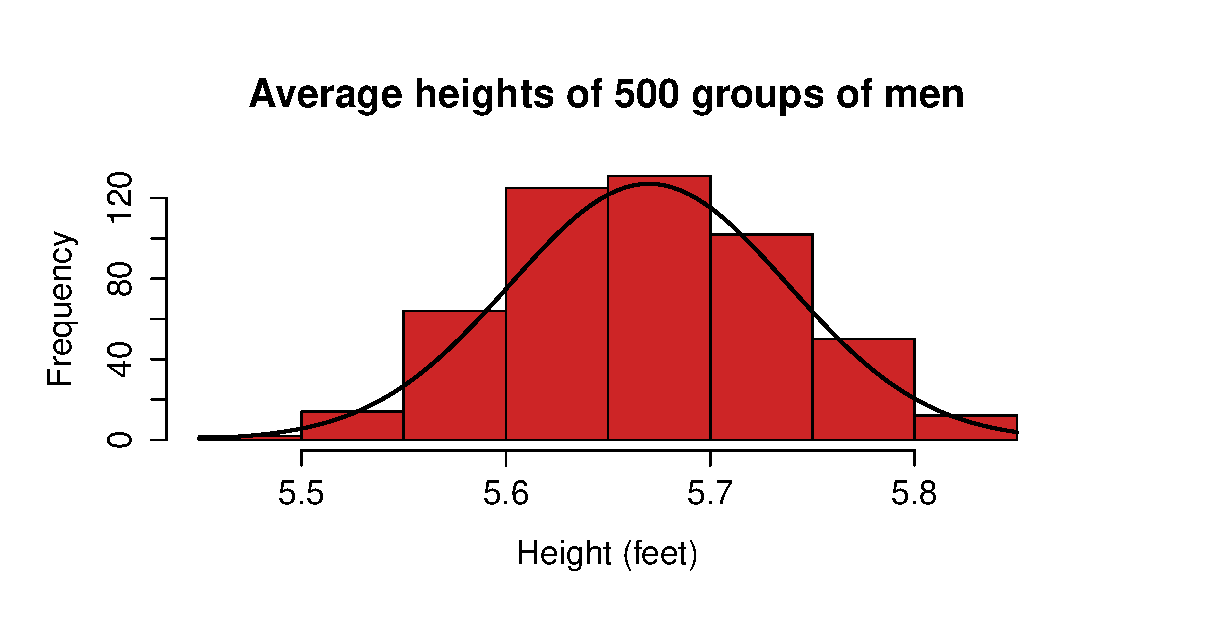
\includegraphics[width=35pc]{uncertainty06}
\caption{Average height of 500 groups of randomly selected men}
\label{fig:uncertainty06}
\end{figure}

All of a sudden, we have a normal distribution with a mean height of 5.67 feet (or 5'8") and a standard deviation of 0.068 feet (or 0.81 inches). We see that the mean of our sampling distribution is exactly equal to the mean of our population: that's the central limit theorem in action.

\subsection{Standard Error}

You might have noticed that the standard deviation of the sampling distribution above was much smaller than the standard deviation of the actual population (0.81 inches versus 4 inches). This arises because we're looking at the variation of a set of means (which themselves are the average value of a larger set of data): these will always vary less than the individual data points that we sample from. And actually, when we're talking about the variation of sample means, instead of standard deviation, we will want to use what's called the \textbf{standard error}, a specific term referring to the standard deviation of a sampling distribution. This will always be smaller than the standard deviation of the population and can be estimated by:

\begin{equation}
\text{SE}_{\bar{x}}= \frac{s}{\sqrt{n}}
\end{equation}

Here, \(s\)  is the sample standard deviation (here, 0.81 inches) and \(n\)  is the number of observations (that is, the number of samples---here, 500). As you can see, the standard error is always going to be smaller than the population's actual standard deviation. In short, the \textbf{standard error} is a measure of how far a sample mean is likely to be from the population mean; the \textbf{standard deviation} is a measure of how far an individual observation is likely to be from the sample mean.

\end{document}